% V0.11 reference catalogue; main.tex does not input this file.
% Active captions and placements are in sections/method.tex and experiments.tex.

\begin{figure*}[t]
\centering
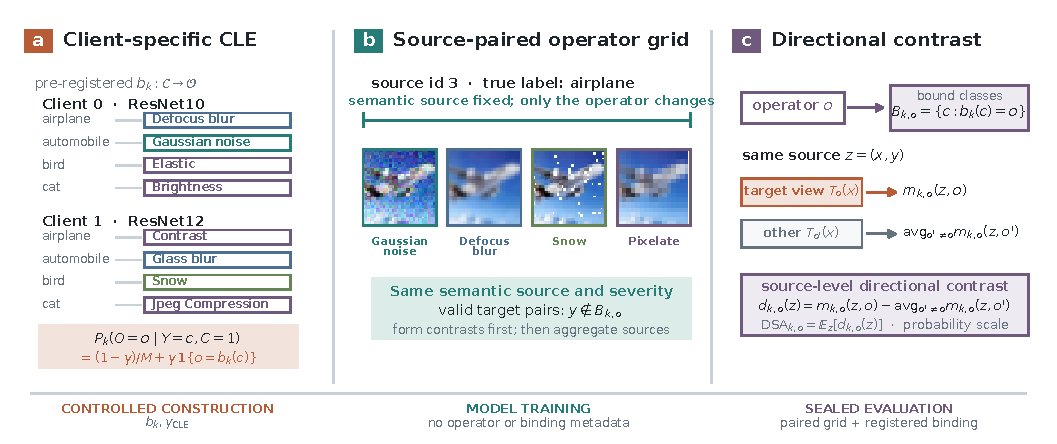
\includegraphics[width=\textwidth,keepaspectratio]{figures/fig_cle_paired_dsa_v4.pdf}
\caption{Client-specific CLE and source-paired DSA diagnosis.}
\label{fig:cle-paired-dsa}
\end{figure*}

\begin{figure*}[t]
\centering
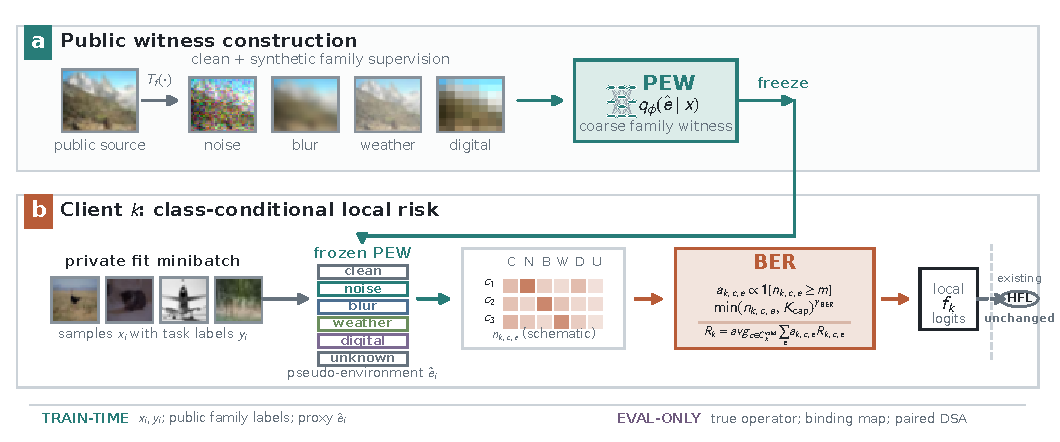
\includegraphics[width=\textwidth,keepaspectratio]{figures/fig_pew_ber_execution_v3.pdf}
\caption{Public PEW and class-conditional local BER execution.}
\label{fig:pew-ber-execution}
\end{figure*}

\begin{figure*}[t]
\centering
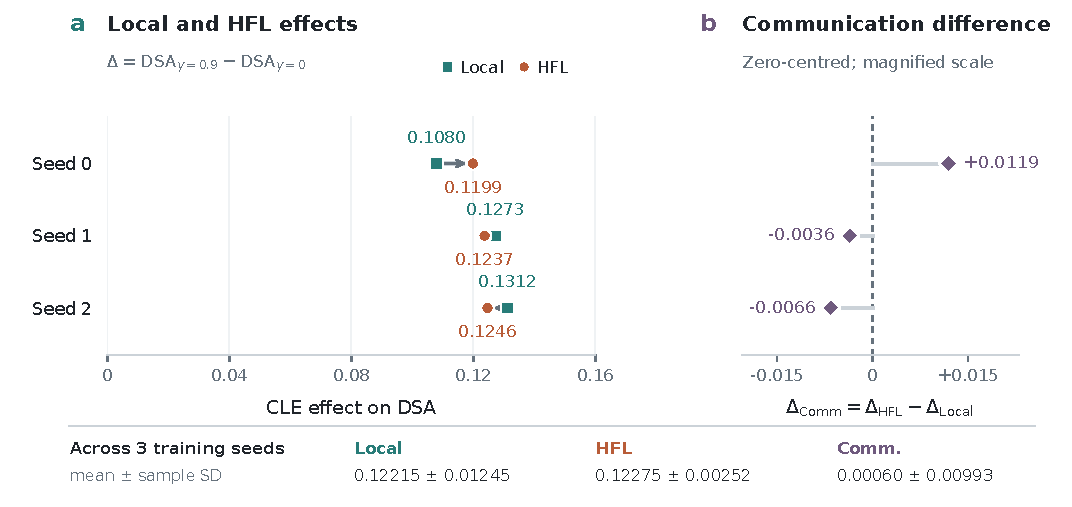
\includegraphics[width=0.96\textwidth,keepaspectratio]{figures/fig_local_first_multiseed_v1.pdf}
\caption{Local-first contrasts; bottom summaries use mean and sample SD across three training seeds.}
\label{fig:local-first}
\end{figure*}

\begin{figure*}[t]
\centering
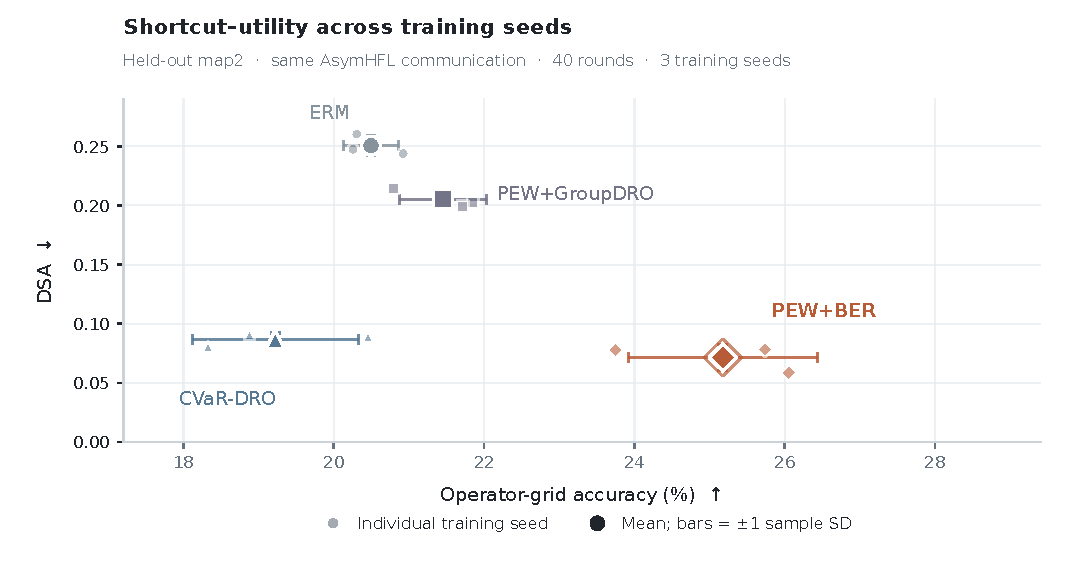
\includegraphics[width=0.94\textwidth,keepaspectratio]{figures/fig_objective_tradeoff_v2.pdf}
\caption{Matched objective comparison with individual training seeds and sample SD bars.}
\label{fig:axis1-objectives}
\end{figure*}

\begin{figure*}[t]
\centering
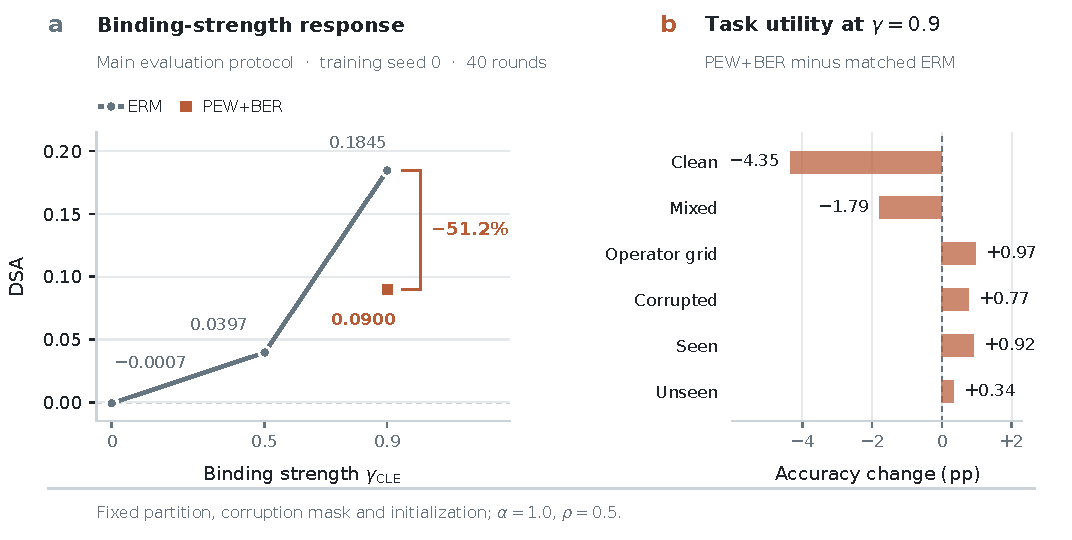
\includegraphics[width=0.96\textwidth,keepaspectratio]{figures/fig_dose_response_v3.pdf}
\caption{Main evaluation dose response and candidate-minus-control utility changes.}
\label{fig:dose-response}
\end{figure*}
